\documentclass[pdf,fyma2]{beamer}
\usetheme{CambridgeUS}

\title{Graph algorithms}
\author{David Svaty}
\institute{ Faculty of Information Technology, BUT }
\date{\today}

\begin{document}
    
\frame{\titlepage}

\begin{frame}
    \frametitle{What is a graph}
    \begin{itemize}
        \item Non-linear data structure
        \item Consists of vertices and edges
        \item Vertices are nodes and edges connect them
        \item Denoted by $G(E,V)$ 
    \end{itemize}
\end{frame}

\begin{frame}
    \frametitle{Graph example}
    \begin{figure}
        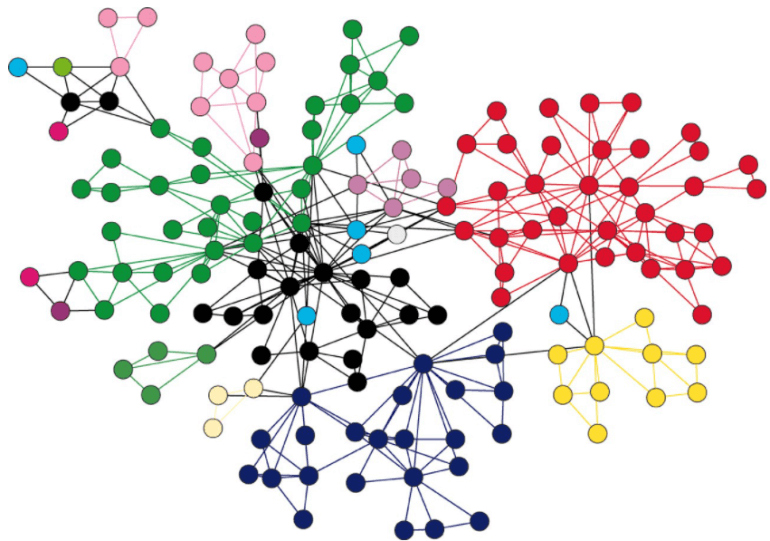
\includegraphics[width=170px]{img/graph-algorithms1.png}
        \caption{Example of a graph. Graph consists of nodes connected by lines.}
    \end{figure}
\end{frame}

\begin{frame}
    \frametitle{Examples of graph algorithms}
    \begin{itemize}
        \item Breadth-first search
        \item Depth-first search
        \item Shortest path
        \item Minimum spanning tree 
    \end{itemize}
\end{frame}

\end{document}